\renewcommand{\theequation}{\theenumi}
\begin{enumerate}[label=\thesection.\arabic*.,ref=\thesection.\theenumi]
\numberwithin{equation}{enumi}
\item The figure \ref{fig:freqpoly1} represents the frequency polygon of two sections.
\begin{figure}[!ht]
\centering
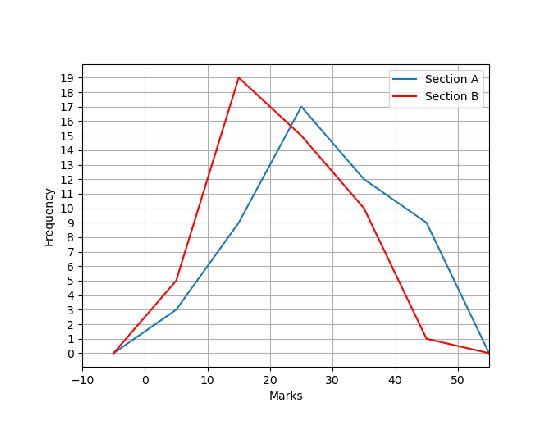
\includegraphics[width= \columnwidth]{./statistics/figs/Q42.eps}
\caption{Frequency polygon of Section A and Section B}
\label{fig:freqpoly1}
\end{figure}
\item From the graph the following can be drawn
\begin{enumerate}
\item Section A has more number of students who got more marks in the range 30-50.
\item Section B has more students in the marks range of 0-20 than Section A.
\item Section A has performed better than Section B.
\end{enumerate}
\end{enumerate}